% !TeX root = ..\..\rapport_13_2.tex
\newpage
\appendix
\appendixpage
\addappheadtotoc
% \begin{landscape}
%     \section{Forfattere}\label{apdx:forfattere}
%     \begin{table}[H]
%         \centering
%         \caption{Oversigt over forfatterskaber i projektet}\label{tbl:forfatter}
%         \begin{tabular}{llllll}
%             \toprule
%             Forfatter         & Afsnit            & Figur & Listing & Tabel & Klasse / Metode                                  \\
%             \midrule
%             Rasmus Wiuff      & \cref{sec:struct} &       &         &       & \mintinline{java}|Eksempel.java|                 \\
%                               &                   &       &         &       & \mintinline{java}|eksempelMetode(String, int[])| \\
%             \midrule
%             Mathies Henriksen &                   &       &         &       &                                                  \\
%             \midrule
%             Max-Emil Scotten  &                   &       &         &       &                                                  \\
%             \midrule
%             Kasper Sylvest    &                   &       &         &       &                                                  \\
%             \bottomrule
%         \end{tabular}
%     \end{table}
% \end{landscape}

% \section{Forfattere}\label{apdx:forfattere}
%     \begin{table}[H]
%         \centering
%         \caption{Oversigt over forfatterskaber i projektet}\label{tbl:forfatter}
%         \begin{tabular}{lll}
%             \toprule
%             Forfatter         & Afsnit             & Filer og klasser                                  \\
%             \midrule
%             Rasmus Wiuff     & \cref{sec:authors}, \cref{sec:struct}, \cref{sec:white_box_generate_project_number},        & \texttt{/facades/...}                 \\
%             \textit{163977}                  &  \cref{sec:contract_generate_project_number}, \cref{sec:solid_d}                       & \texttt{/domain/Activity.java}  \\
%                                           &                         & \texttt{/domain/Report.java}  \\
%                                            &                         & \texttt{/domain/ReportPDFGenerator.java}  \\
%             \midrule
%             Mathies Henriksen  &  \cref{sec:white_box_find_work_time}, \cref{sec:contract_findd_work} , \cref{sec:solid_s},                     & \texttt{/app/...}                                                 \\
%             \textit{s200747}                  & \cref{sec:solid_o}                        & \texttt{/exceptions/...}  \\
%                              &                         & \texttt{/domain/Employee.java}  \\
%                                               &                         & \texttt{/domain/RegularActivity.java}  \\
%                                   &                         & \texttt{/domain/WorktimeRegistration.java}  \\
%             \midrule
%             Max-Emil Scotten   & \cref{sec:white_box_create_initials}, \cref{chap:code_coverage}, \cref{sec:contract_create_initials},                         &  \texttt{/persistency/...}                                                \\
%             \textit{s204633}                 &  \cref{sec:solid_l}                       & \texttt{/viewModels/...}  \\
%                              &                         & \texttt{/domain/ConvertibleToViewModelInterface.java}  \\
%             \midrule
%             Kasper Sylvest    &  \cref{chap:white_box_create_project_activity}, \cref{sec:contract_create_project_activity}, \cref{chap:design},                        & \texttt{/cli/...}                                                 \\
%             \textit{205281}                 & \cref{sec:solid_i}                        & \texttt{/helpers/...} \\
%                              &                         & \texttt{/domain/Project.java}  \\
%                                   &                         & \texttt{/domain/ProjectActivity.java}  \\
%             \bottomrule
%         \end{tabular}
%     \end{table}

\begin{landscape}
    \section{Klassediagram over program laget}\label{apdx:classDiagram_full}
    \begin{figure}[H]
        \centering
        \caption{Klassediagram over program laget}
        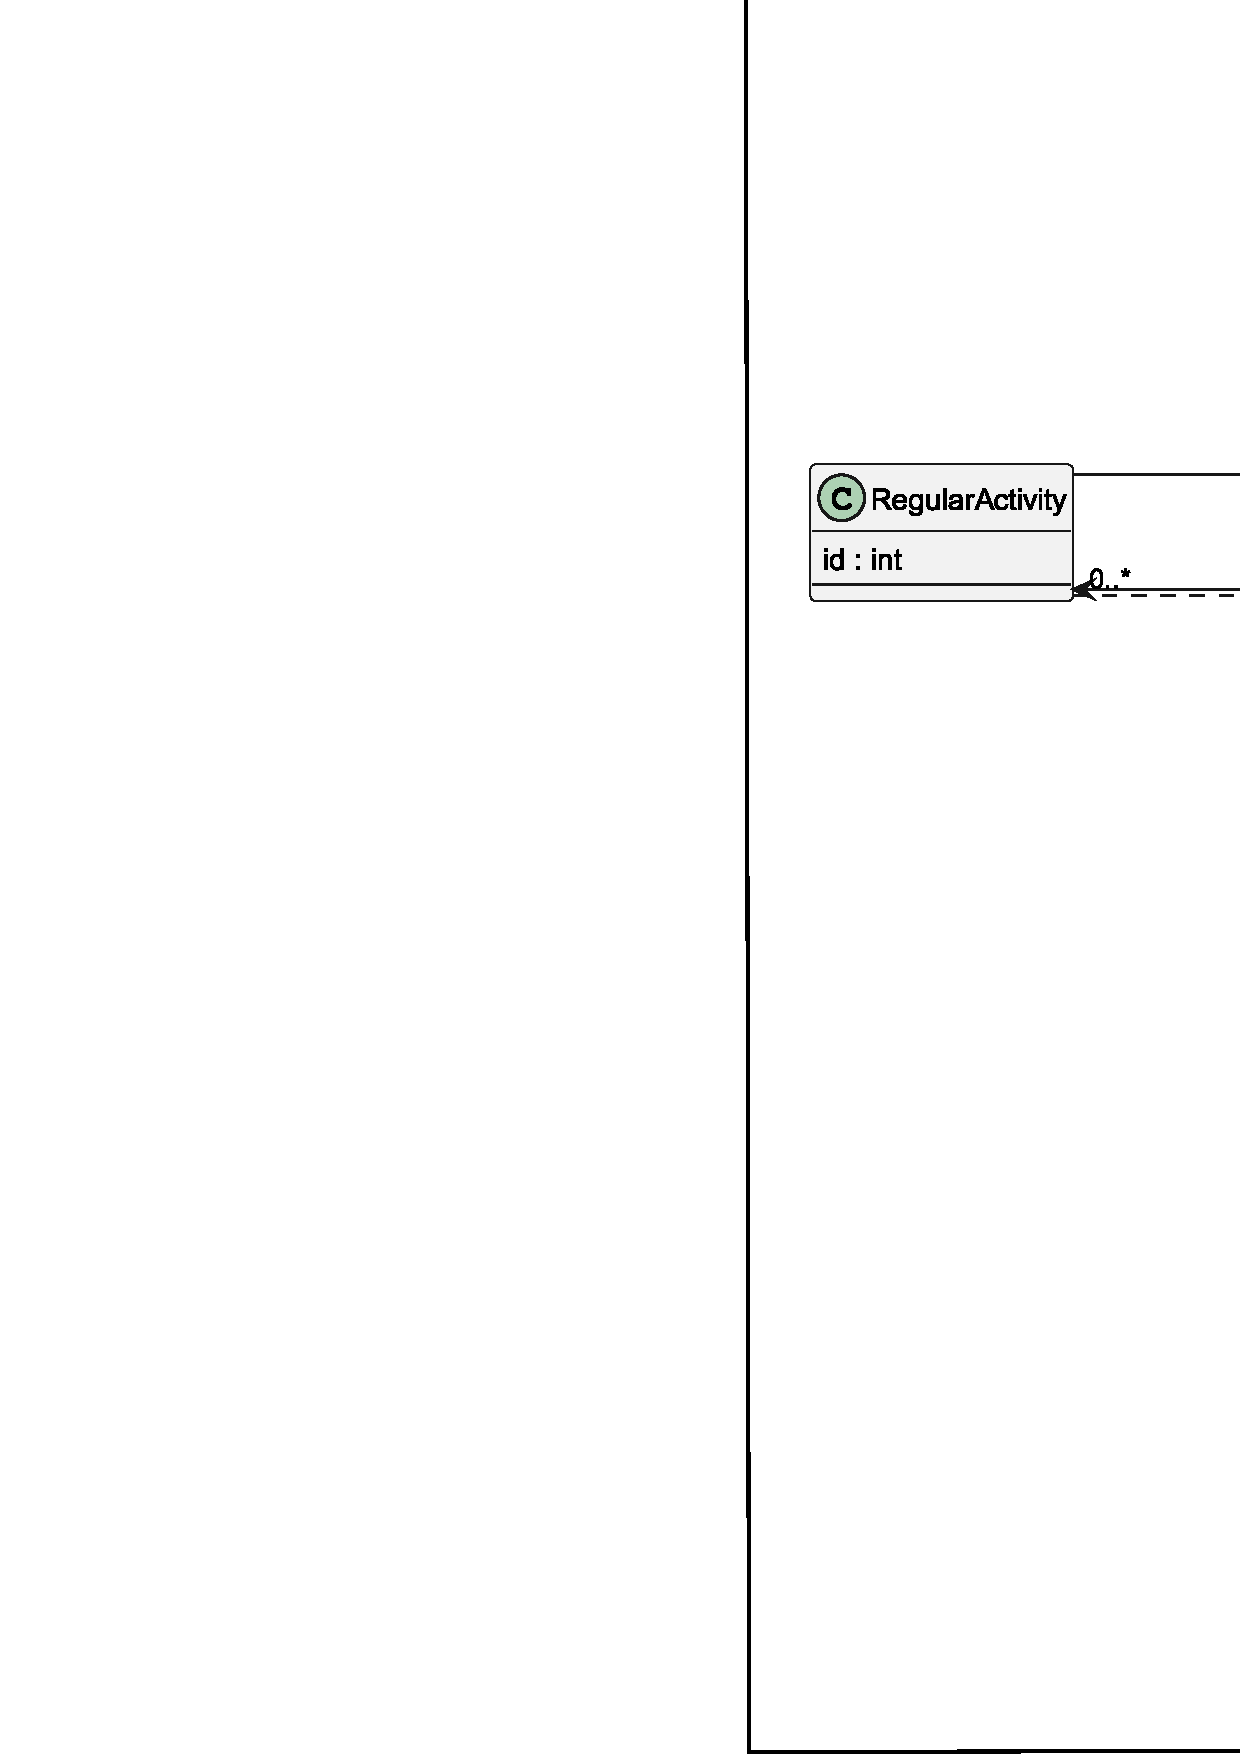
\includegraphics[width = \linewidth, keepaspectratio]{TaskFusion/out/assets/diagrams/class_persistency_full/ClassDiagram_full.png}
        \label{fig:classDiagram_full}
    \end{figure}
\end{landscape}

\begin{landscape}
    \section{Klassediagram over præsentations-laget}\label{apdx:classDiagram_presentation}
    \begin{figure}[H]
        \centering
        \caption{Flowdiagram over CLI brugergrænsefladen}
        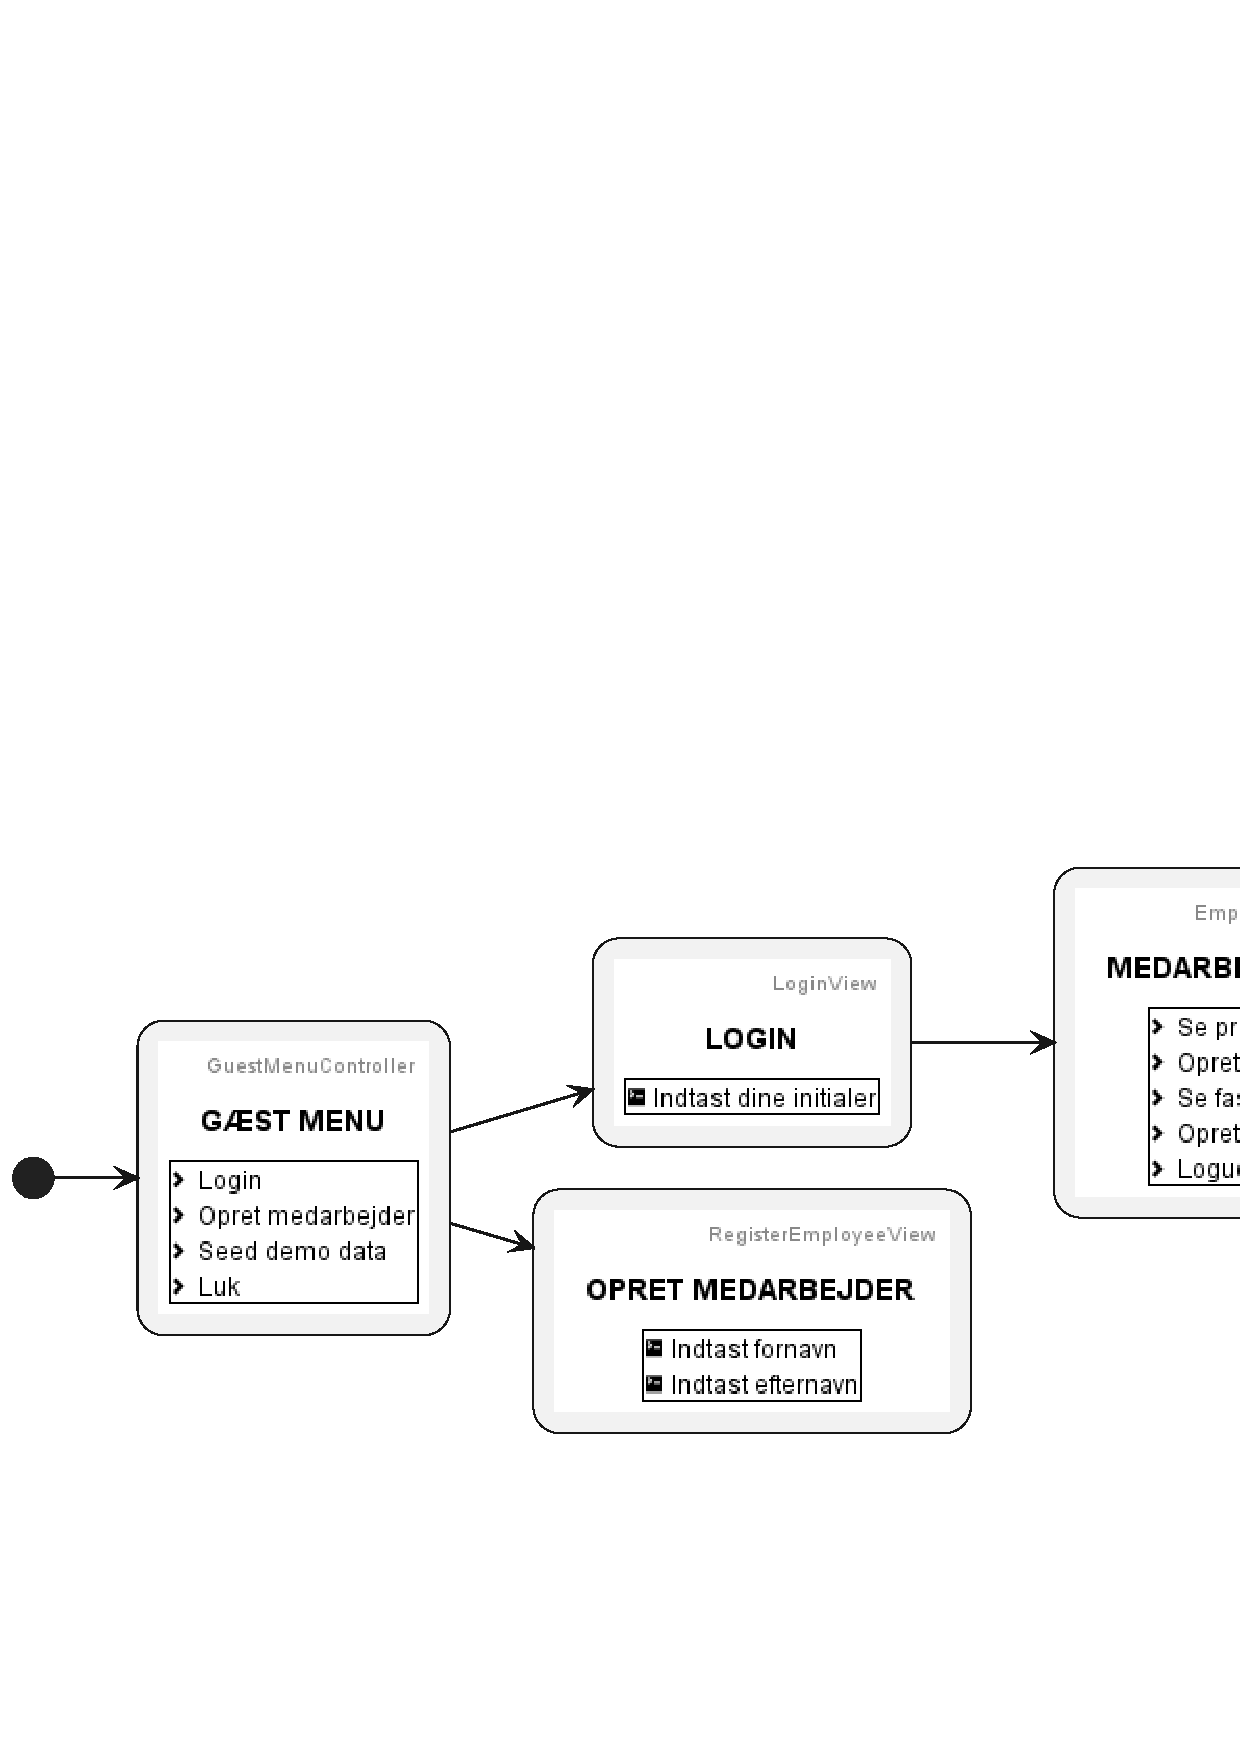
\includegraphics[width = \linewidth, keepaspectratio]{TaskFusion/out/assets/diagrams/flow_cli/flow_cli.png}
        \label{fig:flow_cli_big}
    \end{figure}
\end{landscape}

\begin{landscape}
    \section{Klassediagram over facade-laget}\label{apdx:classDiagram_facade_full}
    \begin{figure}[H]
        \centering
        \caption{Detaljeret klassediagram af facade-laget}
        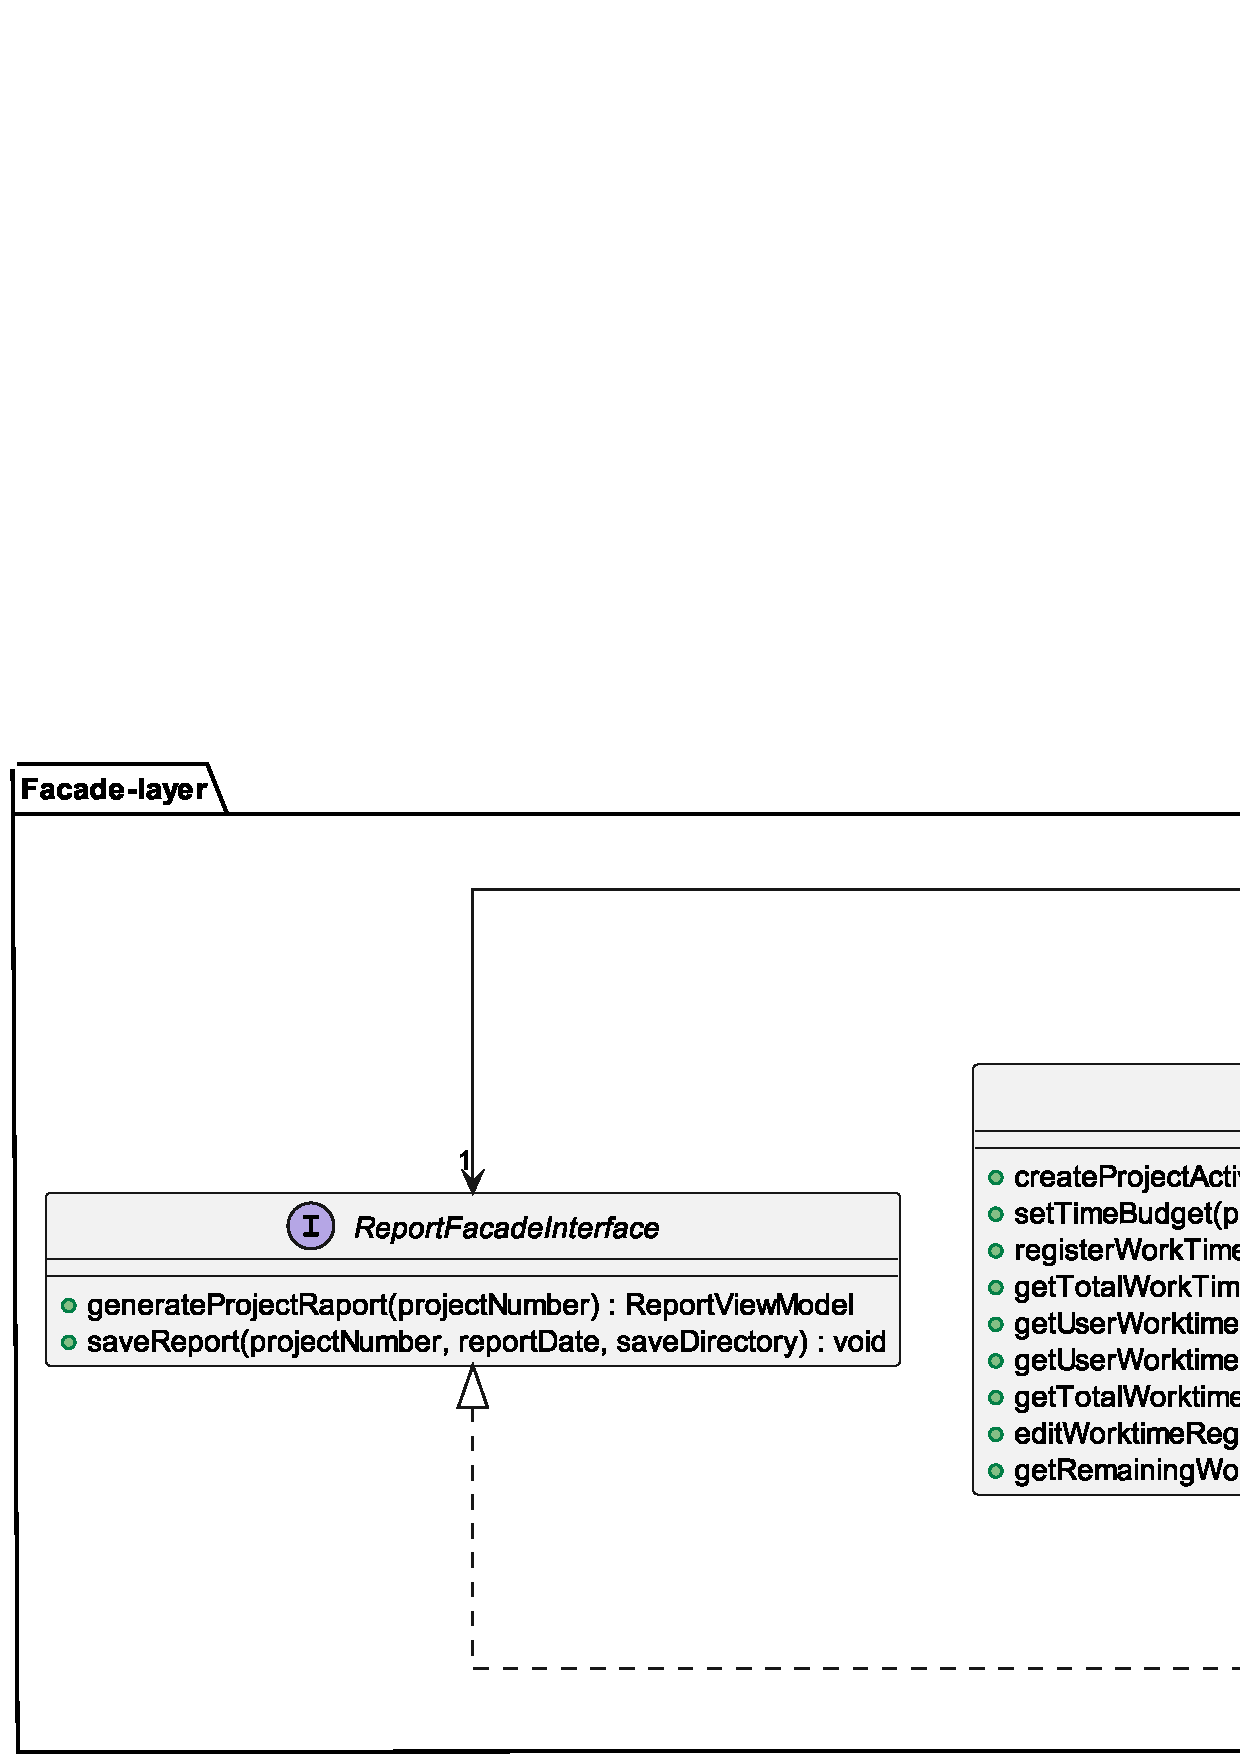
\includegraphics[width = \linewidth, keepaspectratio]{TaskFusion/out/assets/diagrams/class_facade_layer_full/ClassDiagram_facade_full.png}
        \label{fig:class_facade_full}
    \end{figure}
\end{landscape}

